\newchapter{intro}{Introduction}

This is the introductory text.

%\newsection{partPhys}{Particle Physics}

%\newsection{accelIntro}{Particle Colliders}

\newsection{linColliderIntro}{Motivation for Future Linear Colliders}

what colliders are/what they are for

why want a e+ e- collider

why linear better for e+ e-

two proposals - ILC and CLIC. ILC up to 1 TeV. CLIC up to 3 TeV. ILC more mature/could be built now. CLIC more challenging.

\newsection{clicIntro}{CLIC}

basics of main beam, length etc.

accelerating gradient - why need it to be high, why 12 GHz chosen

drive beam - why (efficiency/cost vs. 12 GHz klystrons), combination process, PETS


%\newsection{fontIntro}{FONT}

\newsection{clicPFF}{Phase Feedforward for CLIC}

phase jitter vs. luminosity

expected phase jitter plot

source of phase jitter

proposed layout of system to remove it - turnarounds before extraction. beat timing of beam etc.

required specifications - hardware power, bandwidth, latency etc.

\newsection{ctfIntro}{CTF3}

\subsection{Goals of CTF3}
\label{ss:ctfGoals}

prove main CLIC concepts, drive beam generation, accelerating cavities, etc.

PFF prototype

\subsection{Layout of CTF3}
\label{ss:ctfLayout}

basic parameters: 3GHz/1.5GHz beam, up to factor 8, initial 3-4A, final up to 26A(?)

sections: linac, CT, DL, TL1, CR, TL2, CLEX (TBL/TBTS), CALIFES

\begin{figure}
  \centering
  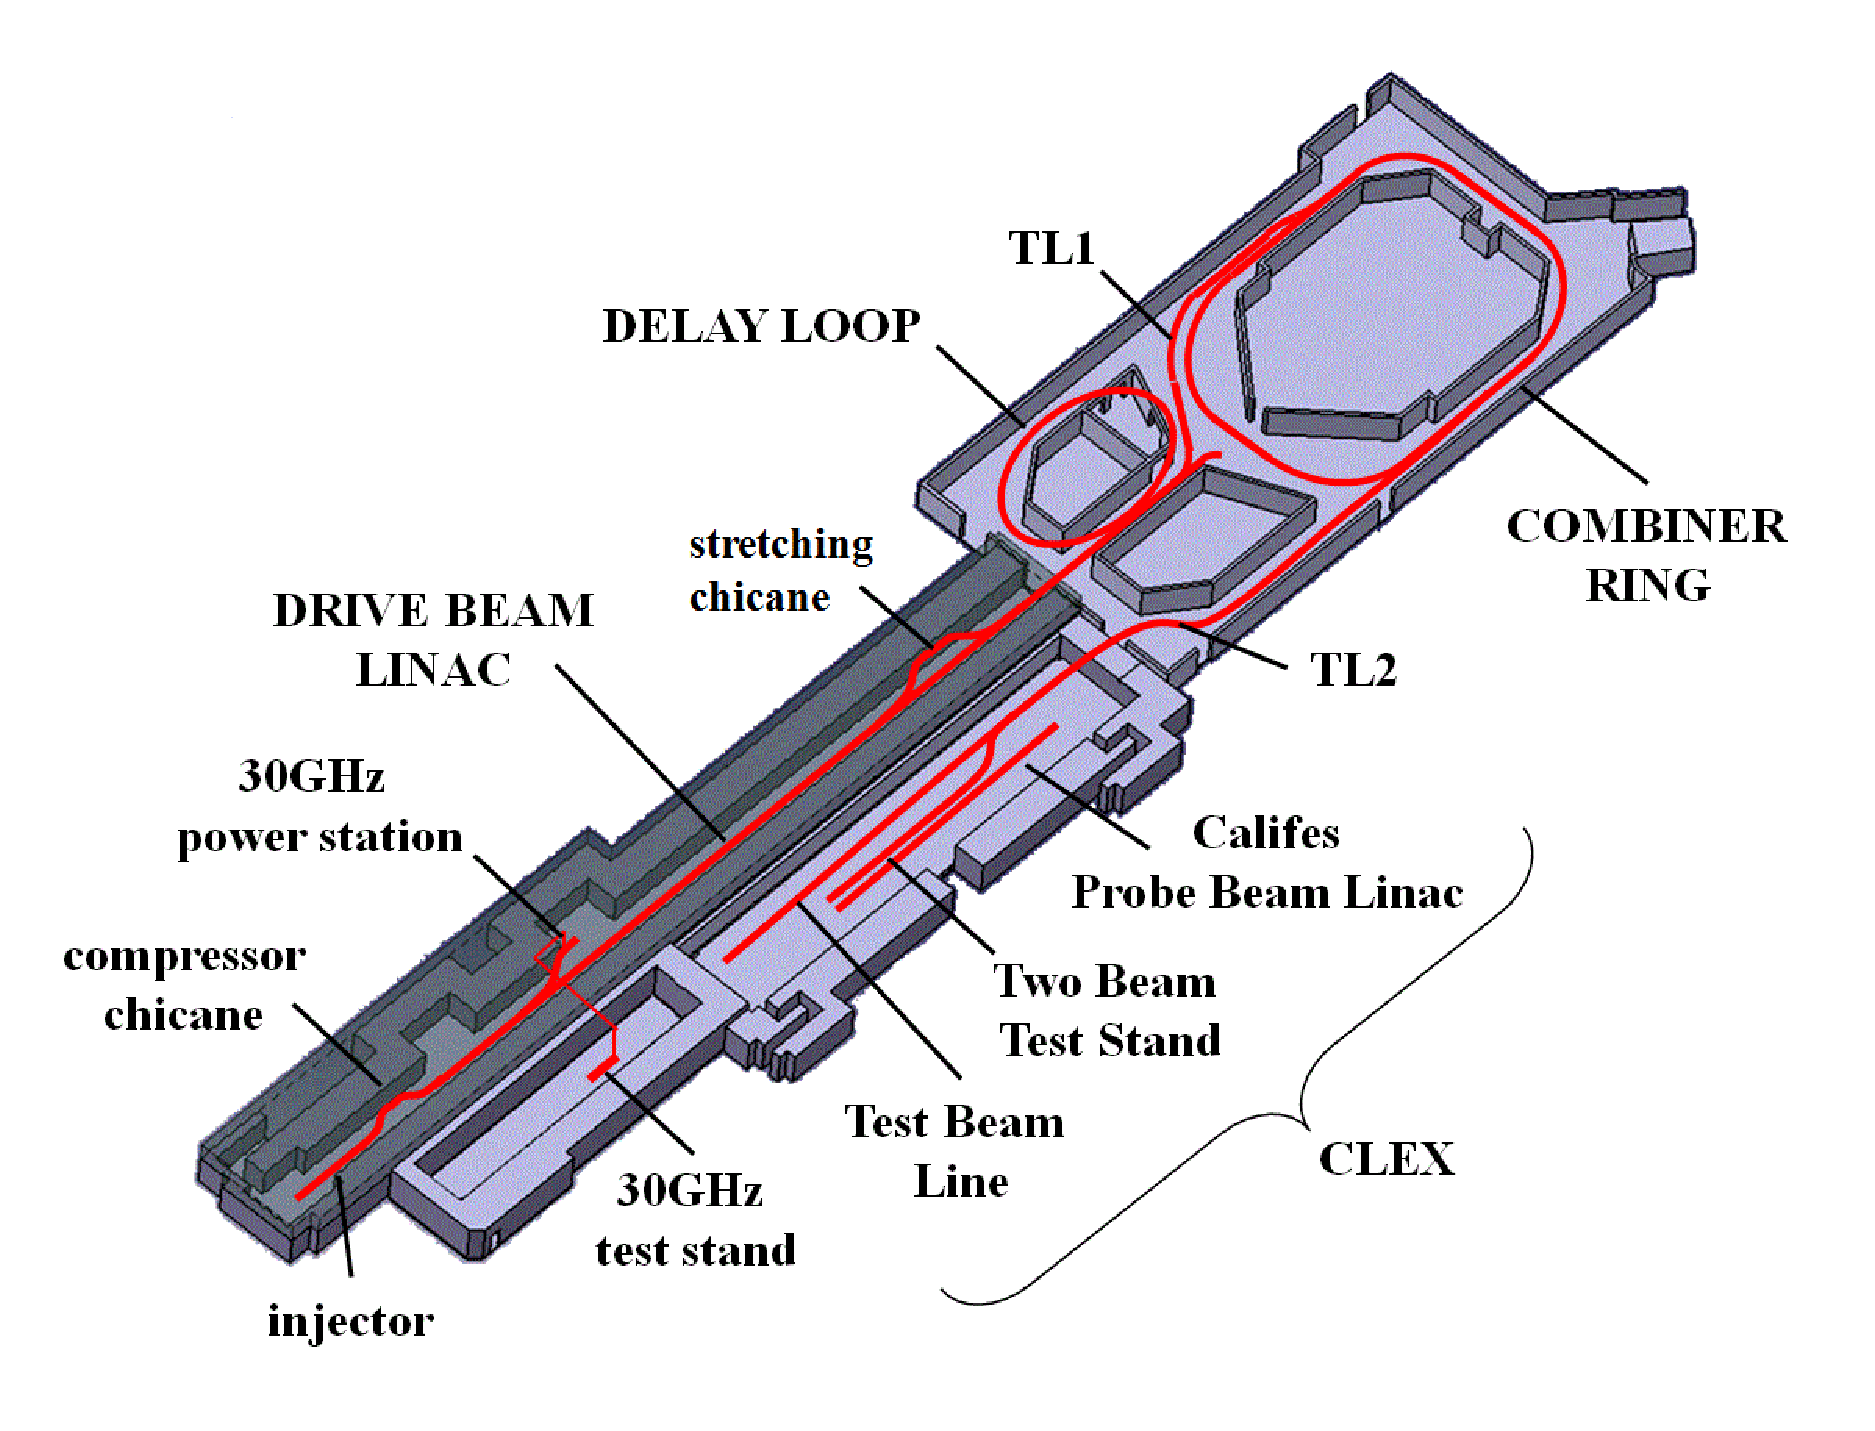
\includegraphics[width=0.45\textwidth]{Figures/ctfLayout}
  \caption{CTF3 schematic.}
  \label{f:ctfLayout}
\end{figure}

\newsection{pffCTFIntro}{Design of the PFF Prototype at CTF3}

\subsection{Schematic Overview of PFF System}
\label{ss:ctfPFFLayout}

location of hardware - CT phase mons, TL2 kickers, TBL phase mon.

diagram of hardware locations

correction range/general targets

\subsection{Hardware}
\label{ss:ctfPFFHardware}

who built the hardware

references to chapters/sections where they are discussed

\subsection{Latency}
\label{ss:availLatency}

beam TOF CT->TL2 chicane

\newsection{ctfVsCLIC}{Differences Between PFF at CTF and CLIC}

operate on uncombined beam
3 GHz
long pulse length - only need to demonstrate stability on combined pulse length for clic

phase sag due to rf pulse compression system - only possible to correct central part of the pulse

\subsection{Phase Sag}
\label{ss:phaseSag}

\subsection{Pulse Length}
\label{ss:pulseLength}

\newsection{phaseJitDefs}{Definitions of Different Phase Statistics}

what I mean by mean phase, phase along pulse, jitter etc.

Definitions of different types of phase jitter.


mean phase

phase along pulse

flatness?

zero phase?


\newsection{thesisOverview}{Thesis Overview}

note that I did not make contribution to hardware design or inital design of PFF system. my first contribution optics.

make point that every chapter shows current status but also highlights areas where improvements can be made for future tests.

quick overview of what each chapter contains:
optics/TL2
phase mons
phase prop
commissioning
results
conclusions



